\chapter{Methodologie}
\label{hst-meth}
Dit hoofdstuk beschrijft hoe de voorgaande theoretische componenten samen een automatische generator van afbeeldingsbeschrijvingen kunnen vormen. De eerste sectie behandelt een bestaande implementatie, die het startpunt vormt van het nieuwe systeem. De volgende secties bekijken uitbreidingen hierop samen met hun implementatie. Concreet moeten deze uitbreidingen zorgen voor verbeteringen op dit startpunt.

Uit de analyse van zinnen gegenereerd door het startpunt blijkt dat, naarmate de zin groeit, het verband met de afbeelding vermindert. Een mogelijke oorzaak ligt in het tegenwerken van twee krachten. Enerzijds moet de beschrijving passen in het taalmodel, anderzijds moet ze de afbeelding zo goed mogelijk beschrijven. Daarom is het doel van de meeste uitbreidingen het toevoegen van extra semantische informatie aan het taalmodel. Op deze manier blijft het model over kennis beschikken van de originele afbeelding. Eerst volgt een bespreking van hoe het mogelijk is om semantische kennis te extraheren uit afbeeldingen met behulp van LDA. De volgende sectie bespreekt de Flickr30k Entities dataset als tweede mogelijke bron van informatie. CCA vormt een derde manier waarbij een multimodale vector deze informatie bevat.

Vervolgens staat dit hoofdstuk stil bij de manier waarop deze informatie kan bijdragen tot de twee gebruikte taalmodellen. Dit kan als vector rechtstreeks in het RNN of als een semantische gids in het LSTM-netwerk. 

De laatste twee secties bespreken twee toevoegingen die geen semantische informatie toevoegen aan het netwerk. De startpuntimplementatie vertoont een voorkeur voor korte zinnen. Daarom beschrijft de voorlaatste sectie een normalisatiemethode voor beam-search. Deze methode is in staat langere zinnen te genereren. Het hoofdstuk sluit af met een beschrijving van Feedforward Sequential Memory Networks, een ander type neuraal netwerk, dat volgens de auteurs ervan veelbelovende eigenschappen heeft.

Figuur~\ref{fig:methodology_overview} toont een overzicht van deze verschillende concepten, samen met de sectie waar ze beschreven staan. Figuur~\ref{fig:system_overview} geeft een schematische weergave van hoe de verschillende beschreven componenten samen een afbeeldingsbeschrijvingssysteem vormen.
\begin{figure}
\centering
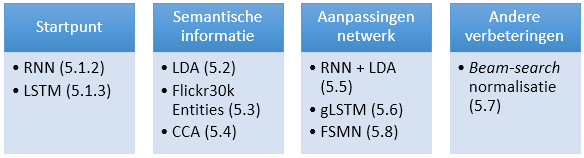
\includegraphics[width=\linewidth]{Images/methodology_overview}
\caption{Overzicht van de concepten uit hoofdstuk~\ref{hst-meth}}
\label{fig:methodology_overview}
\end{figure}

\begin{figure}
\centering
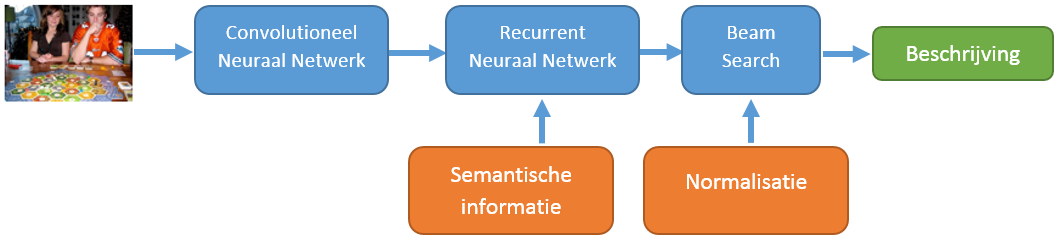
\includegraphics[width=\linewidth]{Images/system_overview}
\caption{Schematische weergave van ons afbeeldingsbeschrijvingssysteem}
\label{fig:system_overview}
\end{figure}



\section{Startpunt}
Het startpunt van onze implementatie is de code aangereikt door Karpathy op zijn GitHub-pagina\footnote{\url{https://github.com/karpathy/neuraltalk}}. Die bevat een Python-implementatie van het recurrente neurale netwerk beschreven in een van zijn papers~\cite{Karpathy2015}. Daarnaast bevat het ook een implementatie gebaseerd op het werk van Vinyals et al.~\cite{Google}. De idee\"en aangebracht in deze masterproef zijn ge\"implementeerd als extensies van dit startpunt.

\subsection{Algemeen systeem}
Karpathy implementeert beide taalnetwerken zelf en voorziet daarrond een gemeenschappelijk systeem. Dit systeem is verantwoordelijk voor het laden en voorbereiden van de data, het maken van tussentijdse back-ups en het aansturen van een \emph{oplosser}. Deze oplosser beheert de netwerken en controleert het trainingsproces.

De netwerken traint hij in batches. Hierbij traint het netwerk niet met steeds \'e\'en voorbeeld, maar met meerdere tegelijk, wat de trainingssnelheid verbetert. 
Hij voorziet verschillende opties om dit gemeenschappelijk systeem te configureren. Hieronder volgt een overzicht van de belangrijkste parameters voor het trainen van het netwerk.
\begin{itemize}
	\item grootte van de verborgen laag van de netwerken
	\item grootte van afbeeldings- en woordcodering
	\item aantal afbeeldingen per batch
	\item type oplosser: rmsprop, Adagrad, Adadelta of gewone gradient descent
	\item afvlakkingsparameter voor rmsprop en Adadelta
	\item epsilon-afvlakking bij rmsprop, Adagrad en Adadelta
	\item al dan niet gebruiken van gradient clipping
	\item drop-out percentage in encoder en decoder
	\item leersnelheid
	\item aantal keer dat een een woord moet voorkomen in de trainingsset, vooraleer het wordt opgenomen in het vocabularium
\end{itemize}
Als CNN gebruikt hij het bestaande vooraf getrainde netwerk VGGNet.

\subsection{Recurrent Neuraal Netwerk}
\label{sec:rnn_methodology}
De eerste implementatie van het startpunt is beschreven door Karpathy~\cite{Karpathy2015}. Hij beschrijft een systeem dat op basis van een afbeelding een beschrijvende zin genereert. Dit gebeurt in twee stappen. Eerst zet een CNN de afbeelding om naar een vectorvoorstelling. Deze vector dient vervolgens als input voor een recurrent neuraal netwerk dat een grammaticaal correcte beschrijving genereert.

\subsubsection{Afbeeldingsrepresentatie}
\label{sec:usedcnn}
Een afbeelding (2D-matrix met een Rood-Groen-Blauw (RGB) waarde voor elke pixel) bevat weinig tastbare informatie. Om dit probleem op te lossen, transformeren de meeste systemen de afbeeldingen eerst naar een vectorrepresentatie. Meestal is deze vector een kansverdeling over verschillende latente concepten uit de afbeelding. Veel van de bestudeerde systemen, waaronder ons startpunt, maken hiervoor gebruik van een convolutioneel neuraal netwerk (CNN).

Het CNN dat momenteel het beste presteert, is VGGNet~\cite{Arge2015}. Dit netwerk heeft implementaties met tot 19 lagen, wat veel meer is dan gebruikelijk op het moment van publicatie. Door het grote aantal lagen kan het netwerk complexere verbanden leren. De lagen bestaan uit groepen van convolutionele lagen afgewisseld met max-pool-lagen, zoals beschreven in sectie~\ref{sec:CNN}.

De laatste lagen van het netwerk zijn volledig verbonden lagen, gevolgd door een softmaxlaag om de output van het netwerk te normaliseren. 

De representatie die Karpathy gebruikt voor afbeeldingen, is de output van de voorlaatste verbonden laag in VGGNet met 16 lagen. Dit leidt tot een 4096-dimensionele vector. Hierbij stelt elke dimensie een bepaald concept voor dat al dan niet aanwezig is in de afbeelding. Deze dimensionaliteit is dezelfde voor alle afbeeldingen, onafhankelijk van de grootte van de input. Dit komt door een herschaling voor de berekening van de afbeeldingsvector.

Aangezien VGGNet momenteel \'e\'en van de best presterende CNN's is op het gebied van afbeeldingsrepresentatie zijn de afbeeldingsvectoren in deze thesis berekend met VGGNet. De berekeningen gebeuren met een publiek beschikbare implementatie in Caffe~\cite{Jia2014}.

\subsubsection{Woordrepresentatie}
Karpathy~\cite{Karpathy2015} stelt vast dat voorgetrainde word embeddings zoals \texttt{word2vec} geen toegevoegde waarde bieden bij het voorstellen van woorden. Om die reden gebruikt hij een one-hotcodering waarbij \'e\'en specifieke code is toegewezen aan het start- en stopwoord. Karpathy kiest ervoor om in zijn model enkel woorden te gebruiken die meer dan vijf keer voorkomen in de trainingsset. Als woorden minder dan vijf keer voorkomen, heeft het systeem te weinig voorbeelden om de betekenis en het gebruik van dit woord te leren. Vooraleer een woord als input dient voor het neurale netwerk, vindt eerst nog een vermenigvuldiging plaats met een gewichtsmatrix $W_{hx}$ en een sommatie met een biasvector. Deze matrix en vector wijzigen mee tijdens het trainingsproces van het netwerk. Op deze manier zijn de semantische verbanden tussen de woordrepresentaties, net als bij word embeddings, toch aanwezig.

\subsubsection{Van afbeelding naar beschrijving}
De berekende vectorrepresentatie van de afbeelding dient als input voor een recurrent neuraal netwerk. Tijdens de training voorspelt het netwerk het eerste woord op basis van de afbeeldingsvector en een speciale vector die de start van een zin voorstelt. Op basis van het gegenereerde woord voorspelt het model dan wat het volgende woord is. Dit proces herhaalt zich tot het einde van de zin bereikt is. Figuur~\ref{fig:rnntraining} toont een eenvoudige weergave van hoe het RNN een beschrijving genereert.

\begin{figure}[tb]
    \centering
    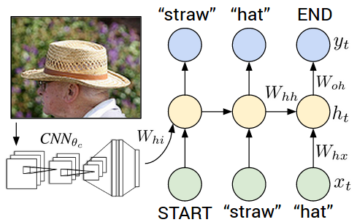
\includegraphics[width=0.5\linewidth]{Images/karpathy.PNG}
    \caption[Generatie van beschrijving met recurrent neuraal netwerk]{Generatie van beschrijving met recurrent neuraal netwerk~\cite{Karpathy2015}}
\label{fig:rnntraining}
\end{figure}

Het trainen van het RNN gebeurt op basis van de Flickr30k dataset. 
Op basis van een willekeurig gekozen afbeelding uit de trainingsset berekent het netwerk de beste zin. Het verschil tussen deze voorspelling en de correcte zin propageert terug door het netwerk en leidt tot de juiste aanpassing van de gewichten.

Evaluatie vindt plaats wanneer de trainingsset volledig is doorlopen. De perplexiteit berekend op de resultaten voor de validatieset geeft snel aan of het netwerk nog bijleert of niet. Deze perplexiteit is een functie van de kans die het taalmodel geeft aan een zin in de validatieset. Voor een zin $X=x_1x_2\dots x_N$ is dit bijvoorbeeld~\cite{Jurafsky:2009:SLP:1214993}:

\begin{equation}
PP(X)=P(x_1x_2\dots x_N)^{-\frac{1}{N}}
\end{equation}

Het systeem slaat de tussentijdse resultaten op in de vorm van \emph{checkpoints}. Deze checkpoints bevatten alle nodige parameters om het opgeslagen model te evalueren. Het is ook mogelijk om de training van het netwerk verder te zetten vanaf een gekozen checkpoint.

Formeel gezien berekent het netwerk op basis van inputvectoren (woorden in de zin) $(x_1,x_2,...,x_T)$ een reeks van verborgen vectoren $(h_1,h_2,...,h_t)$. Deze verborgen vectoren dienen daarna als de basis voor de berekening van de outputvectoren $(y_1,y_2,...,y_t)$. Deze outputs worden verkregen door formules~\eqref{eq:rnnstart}-\eqref{eq:rnnend} te herhalen voor $t = 1$ tot $t=T$.

\begin{eqnarray}
     \vspace{-3mm}
     \label{eq:rnnstart}
     b_v & = & W_{hi} [CNN_{\theta_c}(I)] \\
     \label{eq:rnn}
     h_t & = & f(W_{hx} x_{t} + W_{hh} h_{t-1} + b_h + \delta_{t1} \odot b_v) \\
     y_t & = & sm( W_{oh} h_t + b_o)
     \label{eq:rnnend}
\end{eqnarray}
In deze vergelijkingen zijn $W_{hi}, W_{hx}, W_{hh}, W_{oh}$ en $b_h, b_o$ parameters die het netwerk leert. De $W_{xy}$ zijn gewichtsmatrices, terwijl $b_i$ bias vectoren zijn. $CNN_{\theta_c}(I)$ is de output van de voorlaatste laag van VGGNet met als inputafbeelding $I$. $f$ is een activatiefunctie. $\delta_{t1}$ is de Kroneckerdelta, die waarde $1$ heeft op tijdstip $t=1$ en op andere tijdstippen gelijk is aan $0$. De output $y_t$ is een kansverdeling over de verschillende woorden uit de dataset. Deze kansverdeling bevat ook een extra dimensie voor het END-symbool dat het einde van een zin aangeeft. 

De code van Karpathy maakt bovendien op verschillende plaatsen gebruik van Rectified Linear Units of ReLu-encodering. Deze activatiefunctie zorgt voor effici\"entere gradi\"entpropagatie.

Karpathy schrijft in zijn paper dat het eenmalig gebruiken van de afbeeldingsvector het beste resultaat geeft. Het is ook mogelijk om de afbeelding in elke stap mee te geven. Bij het gebruik van de afbeelding in elke stap verandert formule \eqref{eq:rnn} in formule \eqref{eq:rnnfeedalways}.

\begin{equation}
     h_t = f(W_{hx} x_{t} + W_{hh} h_{t-1} + b_h + b_v)
\label{eq:rnnfeedalways}
\end{equation}

Het genereren van beschrijvingen gebeurt op basis van het \emph{beam-search}-algoritme. Hierbij bepaalt de output van het netwerk de meest waarschijnlijke startwoorden voor de zin. De beste $n$ woorden uit die ranking dienen dan als startpunt van de volgende iteratie. $n$ is hierbij de beam-grootte. Op basis van deze woorden genereert het systeem alle mogelijke opeenvolgingen van twee woorden en voegt deze toe aan de lijst met volledige zinnen bestaande uit \'e\'en woord. Het algoritme gaat door met de $n$ meest waarschijnlijke combinaties, die dus kunnen bestaan uit \'e\'en of twee woorden. Dit proces herhaalt zicht tot alle zinnen een END-symbool voorspellen en dus volledig zijn, of tot het een maximaal aantal iteraties bereikt. De uiteindelijk gegenereerde zin is die met de grootste waarschijnlijkheid.

\subsection{Long Short Term Memory Netwerk}
\label{sec:lstm}
De code van Karpathy implementeert ook een tweede type van neuraal netwerk. Dit netwerk volgt het onderzoek van Vinyals et al.~\cite{Google}. Het betreft een implementatie van een Long Short Term Memory neuraal netwerk. Er zijn wel twee grote verschillen met de paper van Vinyals. Vinyals gebruikt een vergelijkbaar, maar ander type van convolutioneel netwerk. Daarnaast past hij ook ensemble-methodes toe om zo tot het beste resultaat te komen.

De startimplementatie gebruikt net als bij RNN de 4096-dimensionale vectoren berekend met VGGNet als afbeeldingsvoorstelling. Ook de woordrepresentatie blijft dezelfde.

\subsubsection{Van afbeelding naar beschrijving}
Anders dan het RNN van Karpathy, beschouwt deze implementatie de afbeeldingsrepresentatie als het eerste woord in de zin. Daarnaast gebruikt het een LSTM-netwerk als taalmodel, een uitbreiding van een RNN. Op elk moment bevat het netwerk kennis over alle observaties tot op het huidige tijdstip. Door middel van \emph{gates} of poorten is er controle over het al dan niet onthouden van bepaalde waarden. Figuur~\ref{fig:vinyals:karpathy} geeft een schematische weergave van de ontrolling (zoals beschreven in sectie~\ref{sec:rnnconcept}) van het netwerk. Vergelijkingen~\eqref{eq:lstm1}-\eqref{eq:lstm2} geven de nodige berekeningen weer. Hierin is $x_t$ het $t+1$de woord van een zin en loopt $t$ van $0$ tot $N-1$. $W_{hi}$ transformeert de afbeeldingsrepresentatie naar een compactere codering. $p_{t+1}$ is de kansverdeling voor het $t+1$de woord van de gegenereerde zin. De $LSTM$-functie uit de gebruikte formule staat samen met theoretische verduidelijking van het concept in sectie \ref{sub:lstm}. 

\begin{eqnarray}
\vspace{-3mm}
\label{eq:lstm1}
x_{-1} & = & W_{hi}CNN(I)\\
p_{t+1} & = & LSTM(x_t)
\label{eq:lstm2}
\end{eqnarray}

\begin{figure}[tb]
	\centering
	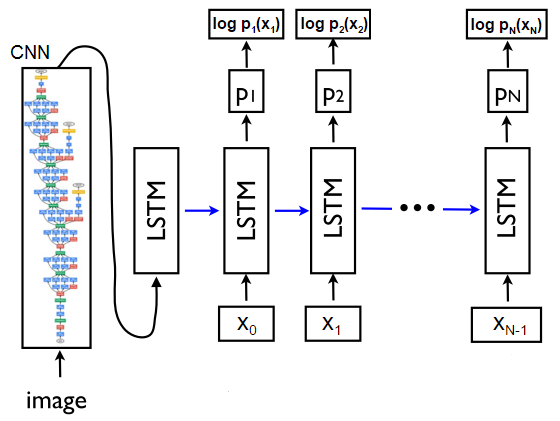
\includegraphics[width=1\linewidth]{Images/vinyals_karpathy.PNG}
	\caption[Ontrold LSTM-model]{Ontrold LSTM-model~\cite{Google}}
	\label{fig:vinyals:karpathy}
\end{figure}

De training van het netwerk verloopt net als bij de RNN-implementatie. Hierbij loopt $t$ van $-1$ tot $N-1$ waarbij het de afbeelding dus als woord $-1$ beschouwt. Het netwerk leert op basis van de Flickr30k trainingsset en bij elk volledig doorlopen van de trainingsset berekent de software de perplexiteit van de resultaten op de validatieset. Dit dient als een criterium om de training stop te zetten en het beste model te bepalen. Hoofdstuk \ref{cha:experimenten} beschrijft een beter criterium voor het vinden van dit beste model.


Het genereren van nieuwe beschrijvingen voor ongeziene foto's gebeurt op exact dezelfde manier als bij RNN. Het \emph{beam-search}-algoritme bepaalt de meest waarschijnlijke zin op basis van de uitkomst van het netwerk.


\section{Latent Dirichlet Analysis}
\label{sec:LDAglobal}
Zoals al kort aangehaald, is het nuttig om tijdens het genereren van zinnen extra semantische informatie aan het netwerk toe te voegen.
Zo biedt het gebruik van Latent Dirichlet Analysis een groot voordeel in de taak van het genereren van nieuwe beschrijvingen. De onderwerpverdelingen bevatten extra semantische informatie die zeer bruikbaar kan zijn voor het genereren van beschrijvingen. Zo is het bijvoorbeeld in staat om geslacht en concrete sc\`enetypes te ontdekken, waar de startimplementatie problemen mee heeft.

Deze sectie beschrijft hoe LDA zorgt voor extra semantische informatie. Dit gebeurt door eerst een model te trainen op de zinnen uit de trainingsset. Vervolgens leert een netwerk LDA-onderwerpverdelingen te voorspellen op basis van afbeeldingsrepresentaties.

\subsubsection{Berekening van LDA-model}
\label{subs:Berekening van onderwerpverdeling}
Het leren van het LDA-model gebeurt op de Flickr30k dataset. Het algoritme om het LDA-model te bepalen beschouwt alle vijf beschrijvingen van een afbeelding na elkaar als \'e\'en document. Net als in het voorbereiden van de data voor het taalmodel, houdt het enkel woorden over die meer dan vijf keer in de trainingsdata voorkomen. Vervolgens verwijdert het bovendien stopwoorden en stemt de woorden met behulp van een \emph{Porter stemmer}. \emph{Stemming} is het reduceren van een woord tot zijn stam. De implementaties van deze voorbereidingstechnieken zijn geschreven met hulpmiddelen uit NLTK\footnote{\url{http://www.nltk.org/}}.

Het doel van dit LDA-model is om op basis van een document te bepalen welke onderwerpen het sterkst aanwezig zijn. Het idee hierachter is dat een onderwerpverdeling ervoor kan zorgen dat het systeem woorden genereert die binnen het juiste onderwerp passen. Het leren van dit model gebeurt met de Python-bibliotheek \texttt{lda}\footnote{\url{https://pypi.python.org/pypi/lda}} en werkt intern met Gibbs sampling.

Het aantal onderwerpen is de belangrijkste parameter van LDA. Het evalueren van een LDA-model is een niet-triviale en moeilijk te automatiseren taak. Om die reden is het bepalen van het beste aantal onderwerpen niet eenvoudig. Enkel indirecte evaluatie biedt de mogelijkheid om de prestatie van LDA te bepalen. Jin et al.\cite{Jin2015} gebruiken ook LDA op dezelfde dataset en gebruiken 80 onderwerpen. Daarom beschouwen de experimenten in hoofdstuk \ref{cha:experimenten} aantallen van onderwerpen rond dit getal. 

Om toch een idee te krijgen over de prestatie van het model gaan we als volgt te werk. Eerst bepaalt een script per onderwerp de tien belangrijkste woorden. Op basis van deze woorden krijgt elk onderwerp een manueel gekozen onderwerpnaam, die een overkoepelend concept voorstelt. Tabel \ref{tbl:woorden-naar-topic} geeft hiervan twee voorbeelden. 
Hierdoor is het enerzijds mogelijk om te kijken of de belangrijkste woorden in een onderwerp een duidelijke link hebben. Anderzijds is het nu ook mogelijk voor elke afbeelding in de trainingsset de vijf meest waarschijnlijke onderwerpnamen op te vragen. Een manuele evaluatie van de onderwerpen per afbeelding geeft opnieuw een idee over de prestatie van het LDA-model. Figuur \ref{fig:ldatopics} toont een voorbeeld van een trainingsafbeelding met de vijf meest waarschijnlijke onderwerpen. Appendix \ref{app:LDA} bevat extra voorbeelden.

\begin{table}
	
	\begin{tabular}{ll}
		Gestemde woorden                                               & Onderwerp \\ \hline
		\texttt{\small{wave man surf ocean surfer ride surfboard person wetsuit board}} & \texttt{surfing}       \\
		\texttt{\small{car truck drive vehicl back van road park driver behing}}        & \texttt{vehicle}      \\
	\end{tabular}
	\caption{Gestemde woorden samen met de zelfgekozen onderwerpnaam}	\label{tbl:woorden-naar-topic}
\end{table}


\begin{figure}[h]
	\centering
	\begin{minipage}[t]{.5\linewidth}
		\centering
		\vspace{0pt}
		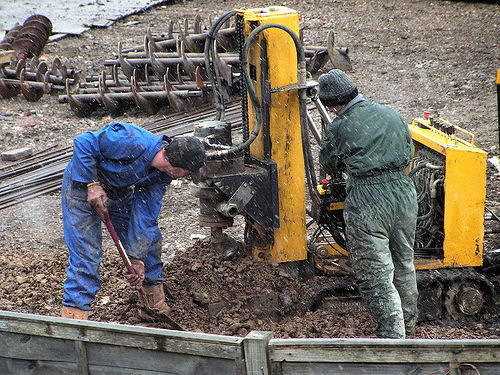
\includegraphics[width=\textwidth]{Images/LDA/5402085.jpg}
	\end{minipage}\hfill
	\begin{minipage}[t]{.5\textwidth}
		\centering
		\vspace{0pt}
		\begin{tabular}{ll}
			Onderwerp                           & Waarschijnlijkheid\\
			\hline
			\texttt{constuctor}             & 0,158 \\
			\texttt{work}                   & 0,113 \\
			\texttt{ground}                 & 0,113 \\
			\texttt{men together}           & 0,113 \\
			\texttt{work/metal/wood}        & 0,047\\
			\hline
		\end{tabular}
	\end{minipage}
	\caption{Voorbeeldfoto met de vijf meest waarschijnlijke onderwerpen}
	\label{fig:ldatopics}
\end{figure}

\subsubsection{Leren van netwerk}
\label{sec:LDAprediction}
Bij invoer van een nieuwe, ongeziene afbeelding moet het systeem een onderwerpverdeling afleiden. De beschrijvingen van de ongeziene afbeelding zijn niet gekend, dus het systeem kan het LDA-model niet rechtstreeks gebruiken. Daarom is er een link nodig tussen een afbeeldingsrepresentatie en een onderwerpverdeling. Een eenvoudig feed-forward neuraal netwerk is in staat om deze link te leggen. 
Het netwerk zorgt voor het transformeren van een afbeelding naar een onderwerpverdeling.

De trainingsverzameling in combinatie met de geleerde onderwerpverdeling vormt de trainingsdata voor dit netwerk. 
Het geleerde LDA-model bepaalt vervolgens de onderwerpverdeling voor de zinnen in de validatieset. Deze onderwerpverdelingen vormen de testverzameling voor het LDA-netwerk. Het doel van het trainen van het netwerk is het verkleinen van de fout tussen de voorspelde verdeling en de berekende verdeling van de validatieverzameling. De fout van het finale netwerk maakt het mogelijk om verschillende configuraties te vergelijken.

Het gebruikte netwerk bestaat uit een inputlaag, een verborgen laag met 256 knopen en een outputlaag. De verborgen laag gebruikt de sigmo\"idefunctie \eqref{eq:sigmoid} als transferfunctie, terwijl de outputlaag een softmaxfunctie gebruikt, zoals besproken in sectie \ref{par:softmax}. Uit experimenten blijkt dat de leersnelheid 0.001 het beste compromis vormt tussen resultaat en snelheid van het leren.
Door middel van terugpropagatie leert het netwerk langzaamaan de juiste gewichten. Dit netwerk kan op het moment van testen zeer snel een onderwerpverdeling bepalen voor een ongeziene afbeelding. Implementatie van het netwerk gebeurde met de Python-bibliotheek \texttt{scikit-neuralnetwork}\footnote{\url{https://scikit-neuralnetwork.readthedocs.org/en/latest/}}.
\begin{equation}
\sigma(t) = \frac{1}{1 + e^{-t}}
\label{eq:sigmoid}
\end{equation}

Wanneer het systeem een ongeziene afbeelding krijgt, gebeurt het volgende: VGGNet zet de afbeelding om naar een vectorrepresentatie. Deze vector dient als input voor de verborgen laag van het neuraal netwerk. Daarna transformeert de softmaxfunctie de output van de verborgen laag naar een kansverdeling over de verschillende onderwerpen. Figuur \ref{fig:learningLDA} toont een visualisatie van dit proces.


\begin{figure}[tb]
    \centering
    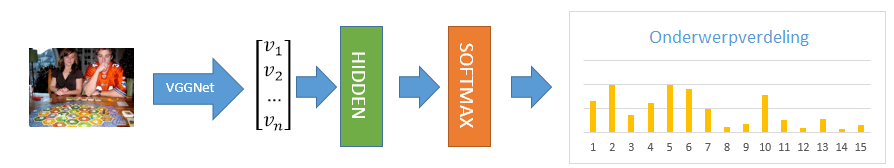
\includegraphics[width=\linewidth]{Images/LDANetwerk.PNG}
    \caption{Het proces om een ongeziene afbeelding te transformeren naar een onderwerpverdeling}
    \label{fig:learningLDA}
\end{figure}

Na de afronding van het trainingsproces moet het netwerk in staat zijn om voor ongeziene afbeeldingen de bijhorende onderwerpverdeling te voorspellen. Dit voorspelde resultaat komt meestal zeer goed overeen met de inhoud van de foto, zoals in figuur \ref{fig:ldalearningexample}. In uitzonderlijke gevallen vertonen de voorspellingen fouten, zoals in figuur \ref{fig:wrongldalearning}. Bij dit voorbeeld is wel duidelijk te zien dat er geen onderwerp is met een grote kans. Bij de correcte voorspelling is er meestal een onderwerp dat een veel grotere waarschijnlijkheid heeft dan de andere onderwerpen. Het valt ook op dat de afbeeldingen waar de voorspellingen slecht zijn overeenkomen met afbeeldingen die in elk bestudeerd beschrijvingssysteem een slechte beschrijving krijgen. Dit komt waarschijnlijk doordat de afbeeldingsvector gemaakt door VGGNet van slechte kwaliteit is. Appendix \ref{app:LDApredictions} bevat meer voorbeelden van correcte en incorrecte voorspellingen.

\begin{figure}[h]
    \centering
    \begin{minipage}[t]{.5\linewidth}
    \centering
    \vspace{0pt}
    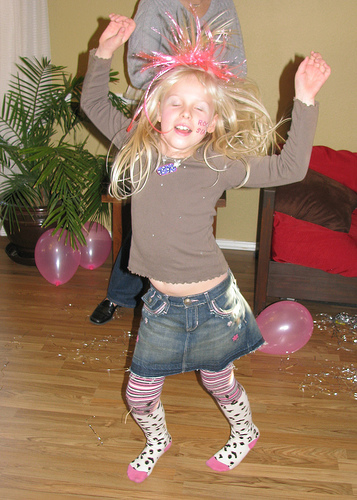
\includegraphics[width=\textwidth]{Images/LDA/2282260240.jpg}
    \end{minipage}\hfill
    \begin{minipage}[t]{.5\textwidth}
    \centering
    \vspace{0pt}
    \begin{tabular}{cl}
            Onderwerp                           & Waarschijnlijkheid\\
            \hline
            \texttt{girl}             & 0,235 \\
            \texttt{dance/perform}                   & 0,096 \\
            \texttt{playground}                 & 0,060 \\
            \begin{tabular}{c}
                \texttt{balloon/}\\
                \texttt{stuffed animal}
            \end{tabular}          & 0,041 \\
            \texttt{children}        & 0,034\\
            \hline
        \end{tabular}
    \end{minipage}
    \caption{Foto met de vijf meest waarschijnlijke onderwerpen -- correcte voorspelling}
    \label{fig:ldalearningexample}
\end{figure}

\begin{figure}[h]
    \centering
    \begin{minipage}[t]{.5\linewidth}
    \centering
    \vspace{0pt}
    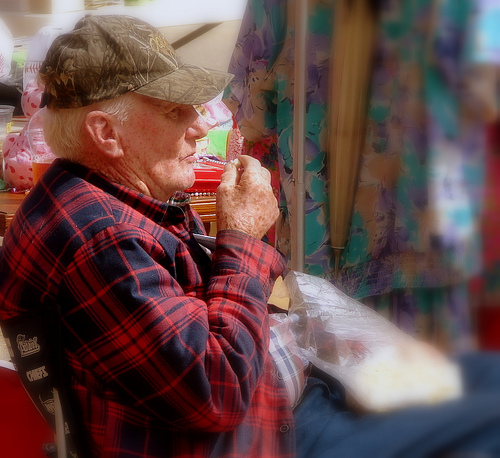
\includegraphics[width=\textwidth]{Images/LDA/3867804763.jpg}
    \end{minipage}\hfill
    \begin{minipage}[t]{.5\textwidth}
    \centering
    \vspace{0pt}
    \begin{tabular}{cl}
            onderwerp                           & waarschijnlijkheid\\
            \hline
            \texttt{musicians}             & 0,039 \\
            \texttt{work}                   & 0,037 \\
            \texttt{baby/toddler}                 & 0,031 \\
            \texttt{clothing}           & 0,027 \\
            \texttt{playground}        & 0,023\\
            \hline
        \end{tabular}
    \end{minipage}
    \caption{Foto met de vijf meest waarschijnlijke onderwerpen -- incorrecte voorspelling}
    \label{fig:wrongldalearning}
\end{figure}


\section{Semantische informatie uit Flickr30k Entities}
De Flickr30k Entities dataset~\cite{Plummer2015}, beschreven in sectie \ref{sec:entities}, bevat extra informatie over de gebruikte foto's. Deze sectie biedt eerst een overzicht van hoe deze informatie nuttig kan zijn. Daarna beschrijft ze de pogingen om deze informatie om te zetten naar een handelbaar formaaat.

\subsection{Nut}
Flickr30k Entities vormt een grote bron aan extra informatie over de afbeeldingen en beschrijvingen uit Flickr30k. Zo is er expliciete kennis over de plaats in een afbeelding waarnaar een woord of woordgroep verwijst. Een netwerk dat deze informatie als extra input heeft, kan hieruit misschien extra informatie leren over bijvoorbeeld de grootte of locatie van bepaalde woorden in de afbeelding. Deze informatie kan ook een verrijking zijn voor het ontdekken van ruimtelijke relaties. Daarnaast verwijzen meerdere frases naar dezelfde omspannende rechthoek. Het is dus mogelijk dat het netwerk semantisch gelijkaardige woorden zoals \texttt{huis} en \texttt{gebouw} als zodanig gaat beschouwen.


\subsection{Gebruik}
\label{sub:Gebruik}
Deze dataset bevat zeer veel extra informatie verspreid over een grote hoeveelheid verwijzingen. Een probleem dat zich voordoet is dat sommige van de omspannende rechthoeken zo klein zijn dat er amper informatie uit te halen is. Daarom is er een reductie uitgevoerd van de dataset alvorens over te gaan tot het verwerken van de data. 

Deze reductie gebeurt op basis van de grootte van de rechthoek. Een deel van de rechthoeken zijn slechts enkele pixels hoog of breed, waardoor een CNN hieruit weinig informatie kan halen. Deze te kleine rechthoeken worden daarom uit de dataset verwijderd. De limiet van zichtbaarheid en informatief zijn van een afbeelding staat ter discussie, maar wij kiezen om alles kleiner dan 64 bij 64 pixels te verwijderen. Dit resulteert in 190.000 omspannende rechthoeken en corresponderende frases. 

De dataset is beschikbaar als tekstbestanden die weergeven welke omspannende rechthoeken op welke afbeelding te zien zijn en met welke delen van de beschrijving elke rechthoek overeenkomt. Er zijn een aantal rechthoeken die wel zijn opgenomen in de dataset, maar geen overeenkomstig zinsdeel hebben. De semantische meerwaarde van dergelijke rechthoeken is miniem, dus behoren deze ook niet tot de bekeken verzameling. 

Om de data bruikbaar te maken voor verwerking leest een script de tekstbestanden uit en slaat alle rechthoeken op als aparte afbeelding. Op basis van die afbeeldingen berekent de Caffe-implementatie van VGGNet een vectorrepresentatie. Een tweede script zet de overeenkomstige zinsdelen om naar een tf-idf gewogen vectorweergave. Deze voorstelling baseert zich op twee belangrijke principes. Ten eerste is het gewicht van een woord in een zin proportioneel met het aantal keer dat het woord $i$ voorkomt in die zin $j$ (term frequentie of $tf_{i,j}$). Ten tweede is het gewicht invers gerelateerd aan het aantal zinnen $n_i$ waar het in voorkomt (inverse document frequentie of $idf_i$). Een woord dat in alle zinnen voorkomt dient een lager gewicht te krijgen dan een woord dat slechts in een fractie van de zinnen voorkomt. Formule~\eqref{formule:tfidf} toont de volledige berekening. Het totaal aantal documenten is hier $N$~\cite{Jurafsky:2009:SLP:1214993}. 

\begin{equation}
\label{formule:tfidf}
	tfidf_{i,j} = tf_{i,j}\cdot{idf_{i}} = tf_{i,j}\cdot{log(\frac{N}{n_i})}
\end{equation}

Op basis van de CCA-uitbreiding beschreven in sectie~\ref{sub:stackedcca} is het mogelijk om een uitgebreide voorstelling te maken van de afbeeldingen uit de Flickr30k dataset. Uit de methodes voorgesteld door Gong et al.~\cite{Gong2014} volgt een representatie van de trainingsafbeeldingen. Deze bevat dan de informatie uit de Flickr30k Entities dataset.

Het berekenen van de CCA projectie tussen de rechthoeken en de frasen uit de Entities dataset verliep zonder problemen. De berekening van de augmentatie ging ook probleemloos, maar het berekenen van de CCA-projectie tussen de augmentaties van de Flickr30k foto's en hun beschrijvingen was qua tijdsbestek niet haalbaar door de hoge dimensionaliteit. Daarom gebruikt geen enkel experiment deze projecties. 

\section{Canonical Correlation Analysis}
Het toevoegen van extra semantische informatie kan gebeuren op verschillende manieren. Een eerste optie is LDA. CCA biedt een tweede mogelijkheid. Waar LDA focust op het blootleggen van verbanden tussen de woorden uit de beschrijvingen, berekent CCA een ruimte die tussen de afbeelding en de zin ligt.

Het berekenen van deze tussenliggende ruimte gebeurt in twee stappen. Een eerste stap is het omzetten van de data naar een bruikbaar formaat. Het eerder vernoemde VGGNet berekent de afbeeldingsvectoren voor de trainingsset. Een tf-idf gewogen vector stelt de bijhorende zinnen voor, zoals eerder beschreven. 

Na het berekenen van de representaties van afbeeldingen en zinnen volgt een berekening van de correlatiecomponenten. Dit gebeurt met de \texttt{MATLAB}-implementatie van het algoritme voor \emph{canonical correlation}\footnote{\url{http://nl.mathworks.com/help/stats/canoncorr.html}}. Het resultaat bestaat uit twee projectiematrices, die dienen om afbeeldings- en beschrijvingsvectoren te projecteren op de tussenliggende ruimte die de correlatie maximaliseert. De experimenten maken enkel gebruik van de projectie voor afbeeldingen, aangezien Jia et al.~\cite{Fernando2015} aantonen dat het gebruik van enkel de afbeeldingsprojectie de beste resultaten oplevert.

Belangrijk is dat de berekening alle zinnen apart beschouwt. Waar de LDA-implementatie de vijf zinnen per afbeelding aaneensluit tot \'e\'en zin, blijven ze hier apart. Een afbeelding kan heel uiteenlopende beschrijvingen hebben waardoor het mogelijk is dat er informatie verloren gaat als het systeem de vijf beschrijvingen als geheel ziet. Meer concreet houdt dit in dat elke foto maximaal moet correleren met elk van de vijf overeenkomstige zinnen uit de trainingsset. Bij het gebruik van LDA zoals in sectie~\ref{sec:LDAglobal} is het aangeraden om de vijf zinnen als geheel te beschouwen. Het doel van het LDA-model is om op basis van een afbeelding \'e\'en onderwerpverdeling te bepalen. Alle vijf zinnen horen bij dezelfde afbeelding en moeten dus samen tot dezelfde onderwerpverdeling leiden.

\section{Toevoeging van LDA-onderwerpverdeling aan RNN}
De eerder berekende LDA-onderwerpverdelingen kunnen dienen als extra semantische informatie om het generatieproces in de juiste richting te sturen. Het integreren van de onderwerpverdeling $L$ in het RNN gebeurt volgens formule~\eqref{eq:rnnldaonce} die~\eqref{eq:rnn} vervangt. Het rode deel in de formule duidt de verschillen met~\eqref{eq:rnn} aan. $W_l$ is een gewichtsmatrix voor vermenigvuldiging met de onderwerpverdeling.

\begin{equation}
    h_t = f(W_{hx} x_{t} + W_{hh} h_{t-1} + b_h + \delta_{t1} \odot b_v \color{red}{+W_lL}\color{black})
    \label{eq:rnnldaonce}
\end{equation}

Het is ook mogelijk om de afbeelding in elke stap toe te voegen, wat leidt tot formule \eqref{eq:rnnldaall}. Het lijkt interessant om te experimenteren met het al dan niet toevoegen van deze informatie in elke tijdstap. De informatie uit de onderwerpverdeling is afgeleid van de afbeelding, maar bevat informatie van een lagere dimensionaliteit. Het herhaaldelijk meegeven van de onderwerpvector zorgt dat het netwerk in elke stap deze semantische informatie binnenkrijgt. Het is dus misschien niet noodzakelijk om de afbeelding in elke tijdstap mee te geven. Hoofdstuk \ref{cha:experimenten} bevat een gedetailleerde beschrijving van de uitgevoerde experimenten en een vergelijking tussen de verschillende instellingen.

\begin{equation}
    h_t = f(W_{hx} x_{t} + W_{hh} h_{t-1} + b_h + b_v \color{red}{+W_lL}\color{black})
    \label{eq:rnnldaall}
\end{equation}


\section{gLSTM}
\subsection{Guided LSTM}
Guided Long Short Term Memory (gLSTM) is een recente uitbreiding van het LSTM-model, ge\"introduceerd door Jia et al.~\cite{Fernando2015}. In dit model extraheren ze eerst semantische informatie uit elke afbeelding. Deze informatie dient als extra input of ``gids'' voor het LSTM-blok.

Na het bestuderen van bestaande LSTM-modellen ontdekten de auteurs dat de gegenereerde zinnen \emph{semantische drift} vertonen. Dit wil zeggen dat naarmate de zin evolueert, de betekenis van volgende woorden steeds minder met de input-afbeelding te maken heeft. Ze vermoeden dat dit komt door twee tegenwerkende krachten. Enerzijds moet de zin de afbeelding beschrijven, anderzijds moet de zin passen in het taalmodel. Om die reden introduceren ze een semantische gids, die ervoor moet zorgen dat het model na enkele woorden op het juiste pad blijft. Dit gebeurt door woorden die semantisch verbonden zijn met de afbeelding een positieve bias te geven.

Ze beschouwen vier verschillende semantische gidsen in hun experimenten. Als eerste model gebruiken ze een \emph{retrieval based} gids. Hierbij zoeken ze eerst naar zinnen die gerelateerd zijn aan de afbeelding. Vervolgens verzamelen ze daaruit de zinnen met de hoogste rang. Deze zinnen vormen dan de extra input.
Als tweede model leren ze eerst een CCA-model. Vervolgens nemen de auteurs de projectie van de afbeeldingsrepresentatie in de gemeenschappelijke ruimte. Daarna zoekt een algoritme de dichtstbijzijnde geprojecteerde zinnen op basis van cosinusgelijkheid. Ook hier vormen de hoogst scorende zinnen de extra invoer.
Een derde model gebruikt de CCA-projectie van de afbeelding in de gemeenschappelijke ruimte rechtstreeks als gids.
Als laatste model gebruiken ze de afbeeldingsrepresentatie zelf als gids.

Om dit te implementeren starten ze net als in deze masterproef met de LSTM-implementatie van Karpathy. Ze defin\"ieren de geheugencellen en poorten zoals in de formules~\eqref{glstm-memory-start}-\eqref{glstm-memory}. Hierbij zijn de rode delen toevoegingen ten opzichte van de standaard LSTM uit formules~\eqref{lstm-memory-start}-\eqref{lstm-memory}.

%
\begin{eqnarray}
\vspace{-3mm}
\label{glstm-memory-start}
i_l' & = & \eta (W_{ix} x_l + W_{im} o_{l-1} \color{red}{+ W_{iq} g}\color{black}) \label{glstm-input} \\
f_l' & = & \eta (W_{fx} x_l + W_{fm} o_{l-1} \color{red}{+ W_{fq} g}\color{black}) \\
u_l' & = & \eta (W_{ox} x_l + W_{om} o_{l-1} \color{red}{+ W_{oq} g}\color{black}) \\
c_l' & = & f_l' \odot c_{l-1}' + i_l' \odot h(W_{cx} x_l + \nonumber \\
&   & + W_{cm} o_{l-1} \color{red}{+ W_{cq} g}\color{black}) \\
m_l & = & u_l' \odot c_l'
\label{glstm-memory}
\vspace{-3mm}
\end{eqnarray}
Hierbij is de gids $g$ de vectorvoorstelling van de semantische informatie. De gids is onafhankelijk van de tijdstap en werkt dus globaal voor elke afbeelding. $W_{iq}$, $W_{fq}$, $W_{oq}$ en $W_{cq}$ zijn extra gewichtsmatrices die het netwerk in de trainingsfase moet leren. Hierdoor vereist elke trainingsstap van dit netwerk meer berekeningen dan de standaard LSTM-implementatie. Figuur \ref{fig:glstm} geeft een visuele voorstelling van het gLSTM-blok.

\begin{figure}[tb]
	\centering
	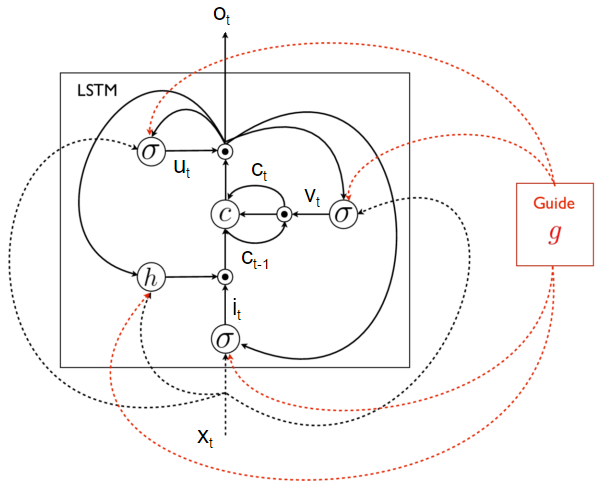
\includegraphics[width=\linewidth]{Images/jia}
	\caption[Schematische weergave gLSTM-blok]{Schematische weergave gLSTM-blok. LSTM-blok in het zwart. Uitbreidingen van gLSTM in het rood~\cite{Fernando2015}.}
	\label{fig:glstm}
\end{figure}

Jia et al. bekomen zeer goede resultaten. De eerste drie gidsen zorgen voor verbetering op hun baseline. Enkel de afbeelding als gids zorgt voor verslechtering. De rechtstreekse CCA-projectie presteert het beste~\cite{Fernando2015}.

\subsection{gLSTM met LDA en CCA}
Net als Jia implementeren we gLSTM als een uitbreiding van LSTM overeenstemmend met formules~\eqref{glstm-memory-start}-\eqref{glstm-memory}.
Om te kunnen vergelijken met hun paper kan de implementatie ook de CCA-projectie van afbeeldingen als gids gebruiken.
Daarnaast veronderstellen we dat LDA-onderwerpverdelingen een goede bron van semantische informatie vormen. Daarom bevat het gecre\"eerde systeem een uitbreiding waarbij LDA de gids vormt van het gLSTM-netwerk.
De experimenten beschouwen zo twee modellen, zodat het mogelijk is om na te gaan welke gids beter presteert in deze configuratie van het gLSTM-netwerk.

\section{Normalisatie van beam search}
Naast het introduceren van gLSTM's breiden Jia et al.~\cite{Fernando2015} de implementatie van Karpathy nog op een tweede manier uit. Na evaluatie van bestaande modellen leiden ze af dat het gebruikte \emph{beam-search}-algoritme een voorkeur heeft voor kortere zinnen. \emph{Beam-search} neemt de som van de logwaarschijnlijkheid van individuele woorden als criterium. Aangezien deze waarde voor elk woord negatief is en het om een maximalisatieproces gaat, zal het algoritme sneller kiezen om te stoppen dan nog een woord toe te voegen. Om dit fenomeen tegen te gaan introduceren ze de genormaliseerde logwaarschijnlijkheid van elk woord als criterium. Concreet leidt dit tot een extra normalisatiefactor $\Omega$ bij de berekening van de waarschijnlijkheid van een woordsequentie (formule~\eqref{eq:log-sentence-norm}).

\begin{equation}
p = \frac{1}{\color{red}{\Omega(\ell)}}\sum_{l=1}^{\ell} \log p(x_l | I, x_{1:l}, \zeta)
\label{eq:log-sentence-norm}
\end{equation}

In deze formule is $\ell$ de lengte van de huidige woordsequentie. $p$ stelt de waarschijnlijkheid voor. $x_i$ is het $i$de woord in de sequentie, $I$ de afbeelding en $\zeta$ zijn de parameters van het taalmodel. 

De auteurs van de paper bestuderen meerdere functies voor $\Omega$. 
De best presterende functie is de Gaussiaanse functie $\Omega(\ell) \sim \mathcal{N}(\mu, sd)$, waar $\mu$ en $sd$ respectievelijk het gemiddelde en de standaardafwijking zijn van de lengtes van de zinnen in het trainingscorpus. Hierdoor moet de lengte van de gegenereerde zinnen gelijkaardig zijn aan die van de zinnen uit de trainingsverzameling. 
Anderzijds bevat onze implementatie \emph{min-hinge}-normalisatie. De normalisatiefactor is dan gelijk aan de gemiddelde lengte van het trainingscorpus ($\mu$) als de zin langer is dan dit gemiddelde. Indien de zin korter is, is de factor gelijk aan de lengte van de zin. Dit komt overeen met de functie $\Omega(\ell)=\min\{\ell, \mu\}$.

Een eigen evaluatie van de gegenereerde zinnen stelt vast dat de zinnen slechts een beperkte woordenschat gebruiken. Daarnaast is er dikwijls een voorkeur voor vage termen, die wel leiden tot een hogere score, maar soms te algemeen of te beperkt zijn.
Om die redenen voegen we een eigen implementatie toe van de $\Omega(\ell)$-functie, die gebruik maakt van $idf$-gewichten. De berekening van deze gewichten baseert zich op het aantal afbeeldingen uit de trainingsverzameling waarbij het woord in kwestie voorkomt in \'e\'en van de vijf beschrijvingen. Alvorens deze gewichten te berekenen zijn de stopwoorden verwijderd uit de trainingszinnen en reduceerde een Porter stemmer alle woorden. De berekende gewichten ($idf_i$) voor elk woord ($w_i$) komen dan overeen met volgende formule: 


\begin{equation}
    idf_i = \log(\frac{N}{n_i})
\end{equation}
Hierbij stelt $N$ het aantal afbeeldingen voor en staat $n_i$ voor het aantal afbeeldingen waar het woord $w_i$ voorkomt in de beschrijvingen.

Deze gewichten vertonen een verband met de hoeveelheid informatie die het woord bevat. De woorden met laagste en hoogste $idf$-score staan respectievelijk in tabel \ref{tbl:idf-laag} en tabel \ref{tbl:idf-hoog}. Om een normalisatie te verkrijgen, telt het algoritme de gewichten voor alle afzonderlijke woorden op. Op deze manier is er een afstraffing voor zinnen die veel frequente woorden bevatten en dus minder veelzeggend zijn. Anderzijds zorgt dit er ook voor dat er niet langer een voorkeur is voor korte zinnen.


\begin{table}[!htb]
	\begin{minipage}{.5\linewidth}
		\centering
		\begin{tabular}{ll}
    man    & 1.099 \\
    two    & 1.946 \\
    woman  & 1.946 \\
    people & 2.198 \\
    shirt  & 2.303 \\
		\end{tabular}
		\caption{Woorden met laagste $idf$}
		\label{tbl:idf-laag}
	\end{minipage}%
	\begin{minipage}{.5\linewidth}
		\centering
		
		\begin{tabular}{ll}
	fingerless & 10.275\\
	creamer& 10.275\\
	vigor& 10.275\\
	ghetto& 10.275\\
	raceway& 10.275\\
		\end{tabular}
		\caption{Woorden met hoogste $idf$}
		\label{tbl:idf-hoog}
	\end{minipage} 
\end{table}


\section{FSMN}
E\'en van de eerste wijzigingen die we in deze thesis probeerden te implementeren, waren Feedforward Sequential Memory Neural Networks (FSMN)~\cite{Zhang}. Deze netwerken vormen een uitbreiding op gewone feed-forward neurale netwerken. Dit netwerk kan afhankelijkheden op lange termijn leren zonder recurrente verbindingen te gebruiken. Het doet dit door het gebruik van sequenti\"ele geheugenblokken in de verborgen lagen van het feed-forward netwerk. 

Volgens de paper zijn deze netwerken in staat om betere en vooral snellere resultaten te leveren dan de huidige RNN-modellen. De snellere resultaten zijn mogelijk omdat gebruik kan worden gemaakt van standaard terugpropagatie zonder dat er zich problemen voordoen bij de recurrente verbindingen. Figuur~\ref{fig:fsmn} toont de  algemene structuur van dit netwerk. Hierbij dient de output van een verborgen laag als input voor een geheugenblok. Dit geheugenblok is in staat om informatie bij te houden van meerdere vorige inputs. Het geheugenblok dient ook als extra invoer voor een volgende laag.

Vooral de snellere resultaten leken zeker een goede uitbreiding voor het model van Karpathy. Trainen van een RNN-batch duurt ongeveer 4 seconden en een LSTM-batch duurt 7 seconden. Hierdoor duurt het volledig trainen van het neuraal netwerk gemiddeld meer dan zeven dagen.
Hoewel de implementatie van dit netwerk op basis van de paper succesvol was, vertonen de resultaten zowel op vlak van kwaliteit als snelheid geen verbetering. De oorzaak van het kwaliteitsverlies ligt in het gebruik van het aantal lagen. Aangezien het gebruikte RNN van Karpathy slechts \'e\'en verborgen laag heeft, is de verbetering door het omzetten naar een FSMN miniem. FSMN's werken slechts beter als er meerdere verborgen lagen zijn. Het aantal verborgen lagen heeft ook een invloed op de verbetering op vlak van snelheid. Bij een klassiek RNN zorgt een toename van het aantal lagen voor meer terugkoppelingen en dus langere rekentijden. Een FSMN heeft dit probleem niet, en presteert dus sneller in verhouding tot een RNN met evenveel verborgen lagen, maar enkel bij het gebruik van meerdere verborgen lagen. Bij het gebruikte RNN is de verbetering dus niet zichtbaar, aangezien er slechts \'e\'en verborgen laag is. Om deze redenen waren er geen verdere experimenten met FSMN's.

\begin{figure}[tb]
	\centering
	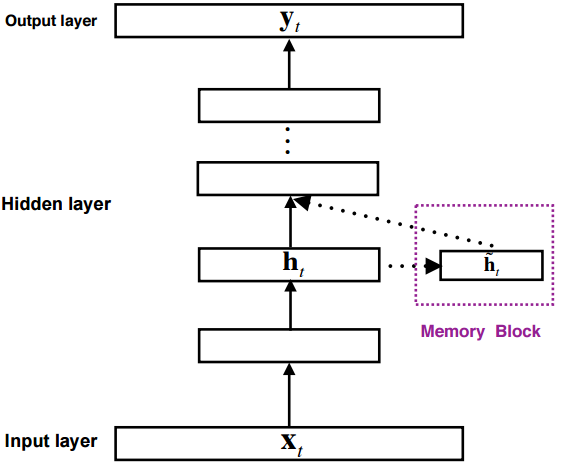
\includegraphics[width=0.6\linewidth]{Images/fsmn_ours}
	\caption{Algemene structuur van Feedforward Sequential Memory Neurale Netwerken.}
	\label{fig:fsmn}
\end{figure}

\section{Besluit}
Op basis van de theorie uit hoofdstuk~\ref{hst-theorie} bouwt dit hoofdstuk een systeem dat kan bestaan uit verschillende componenten. De basis hiervoor ligt bij een bestaande implementatie. Deze implementatie gebruikt een CNN om afbeeldingen om te vormen tot een vectorvoorstelling. Deze voorstelling dient als invoer voor een neuraal netwerk dat als taalmodel dienst doet. Dit netwerk kan een RNN of een LSTM zijn. Vervolgens zijn er verschillende manieren om de prestatie van deze basisnetwerken te verbeteren.  Een vector met een onderwerpverdeling (LDA) of een projectie van de afbeelding (CCA) kunnen zorgen voor extra semantische informatie. Om verbetering aan te brengen in de gegenereerde zinnen implementeren we drie types van normalisatie van het beam-search-algoritme dat de zinnen vormt. Een aantal onderzochte technieken zijn door computationele complexiteit of gebrek aan verbetering niet opgenomen in de experimenten. 

Om deze systemen te kunnen vergelijken zijn er methodes nodig die op een objectieve manier evalueren hoe modellen presteren. Het volgende hoofdstuk biedt een overzicht van de verschillende evaluatiemogelijkheden.